
% Radar Thời tiết
\vspace{2cm}
\begin{figure}[H]
    \centering
    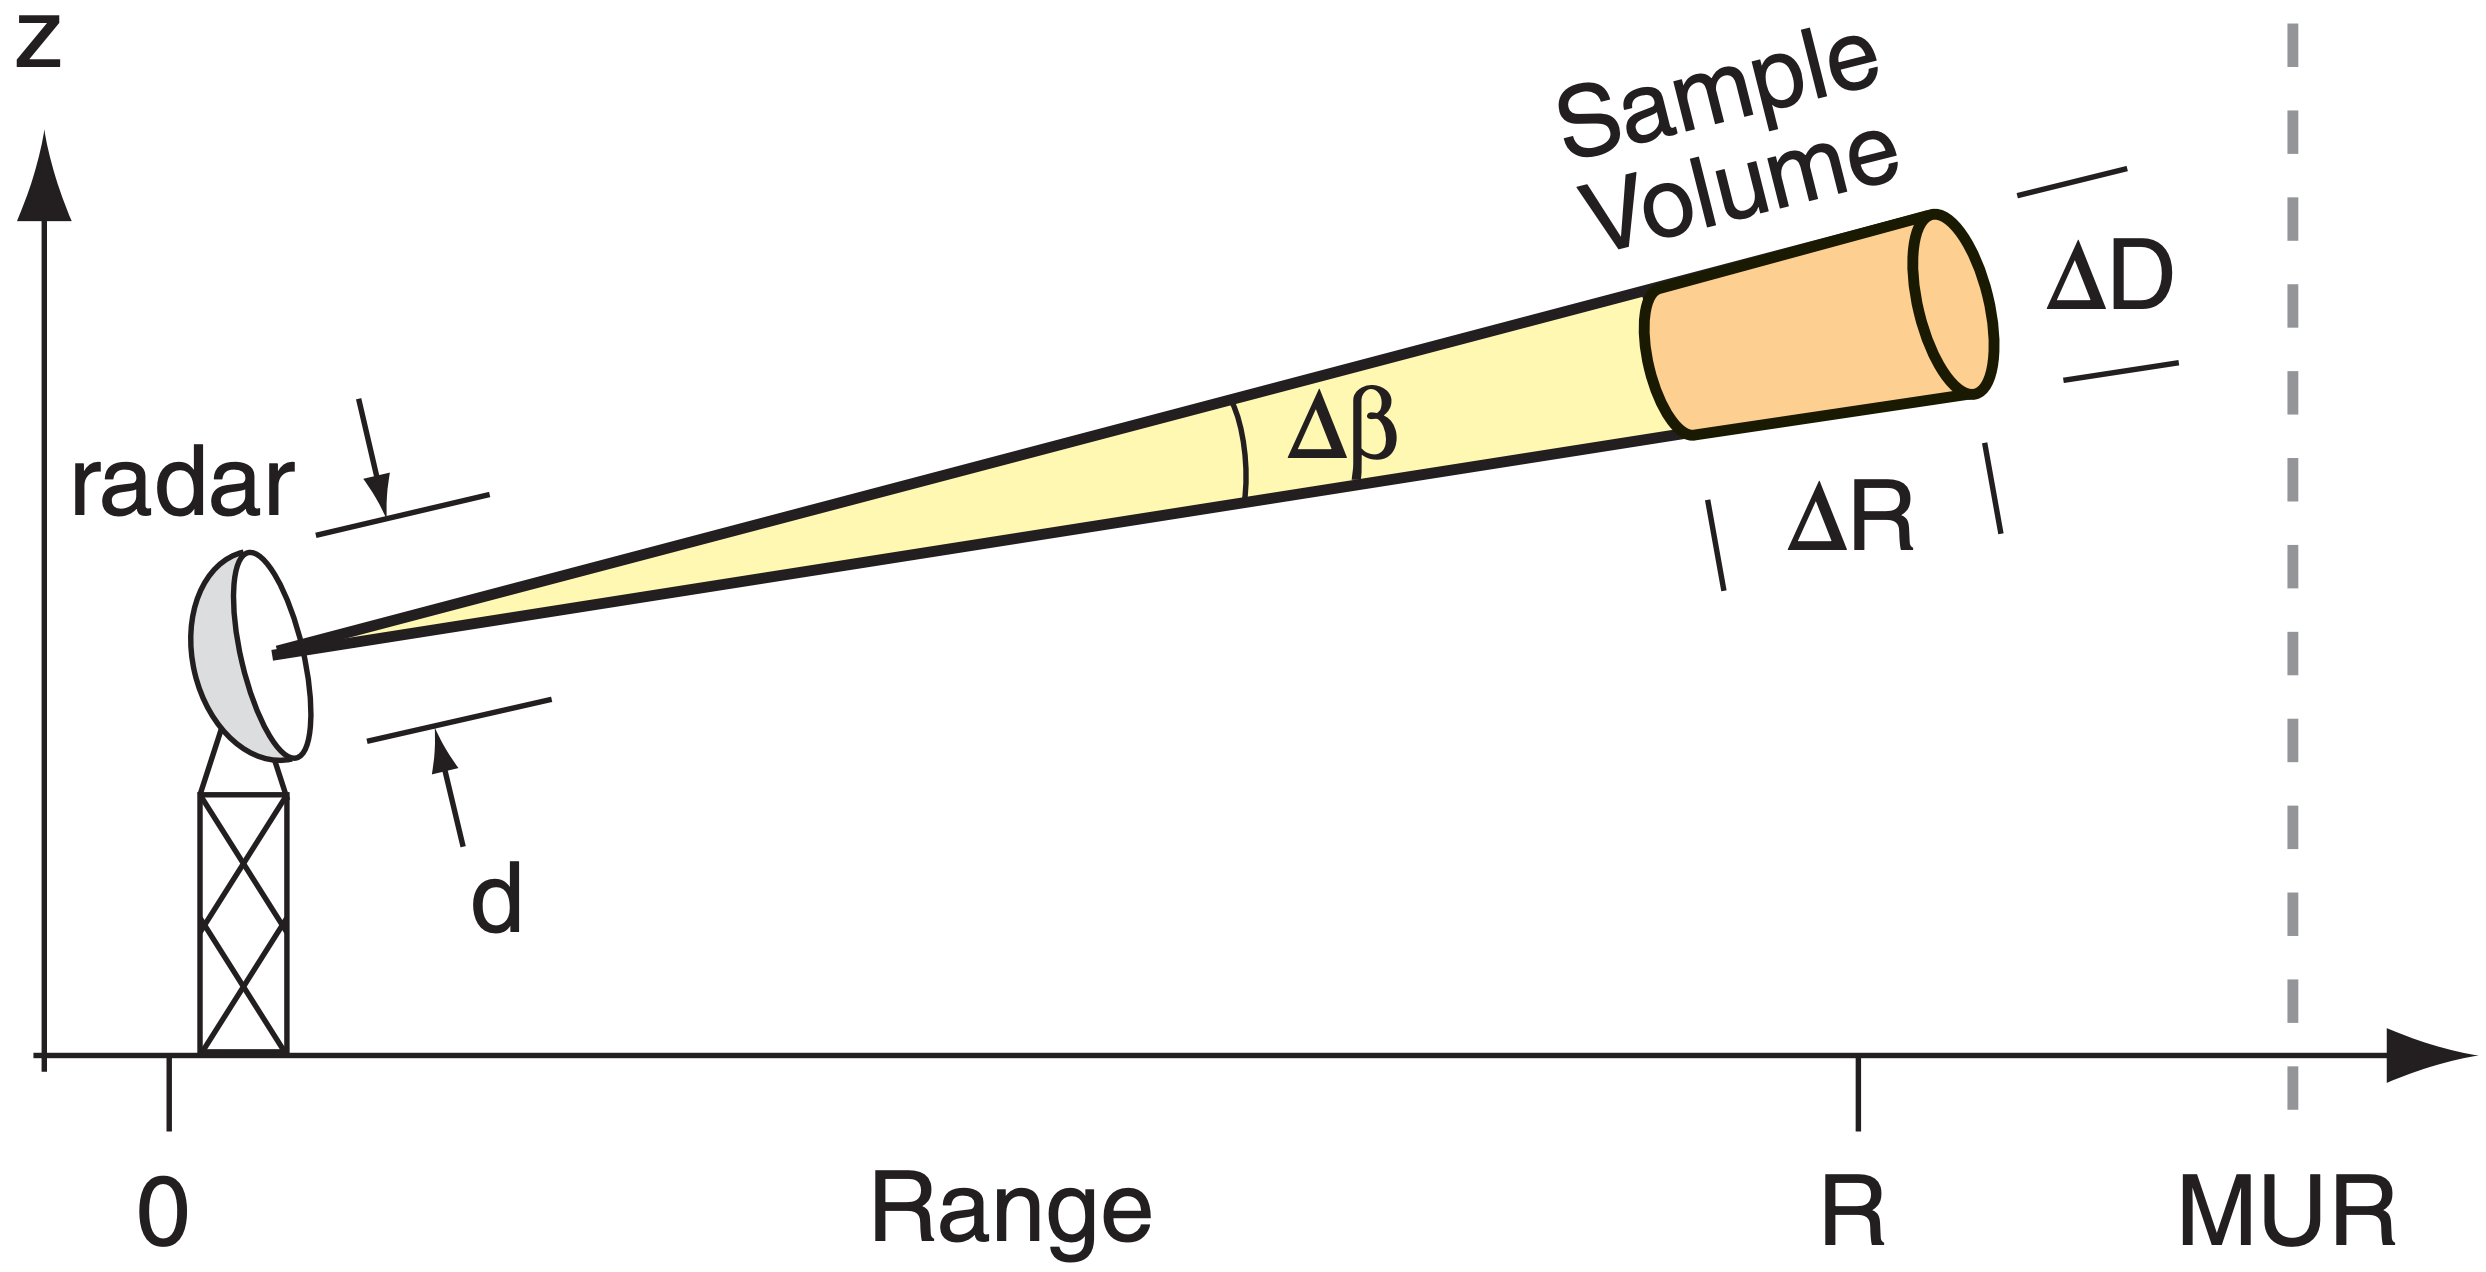
\includegraphics[width=1\linewidth]{Images/radar_concept.png}
    \vspace{1em}
    \caption{Hệ thống radar thời tiết - \cite{2022Weather}}
    \label{fig:radar}
\end{figure}
\newpage
% Các khái niệm cơ bản
\subsection{Các Khái Niệm Cơ Bản}


\subsubsection{Radar thời tiết}
\footnote{Tên tiếng Việt của các thuật ngữ sẽ được căn cứ dựa trên TCVN 12636-12 : 2021 \cite{vn_meteor_standard}}
Radar thời tiết là một loại cảm biến có khả năng phát sóng vô tuyến (bước sóng trong phạm vi từ 250 - 1000 kW) \cite{2022Weather}. Để gia tăng cường độ sóng, một chảo antent (attenna dish) hình parabol được sử dụng nhằm hội tụ bước sóng. Radar có thể nâng và hạ (tuỳ theo yêu cầu) để thu nhập thông tin tại các vị trí chỉ định trong không gian 3 chiều.

Thông thường, các radar được lập trình để quét theo góc hướng (azimuth) $360^o$, mỗi vòng sẽ quét ở một gốc nâng khác nhau. Như vậy, radar sẽ mất khoảng từ 4 đến 10 phút để hoàn thành một lần quét.

\begin{figure}[htp!]
\centering
\begin{subfigure}{\textwidth}
    \centering
    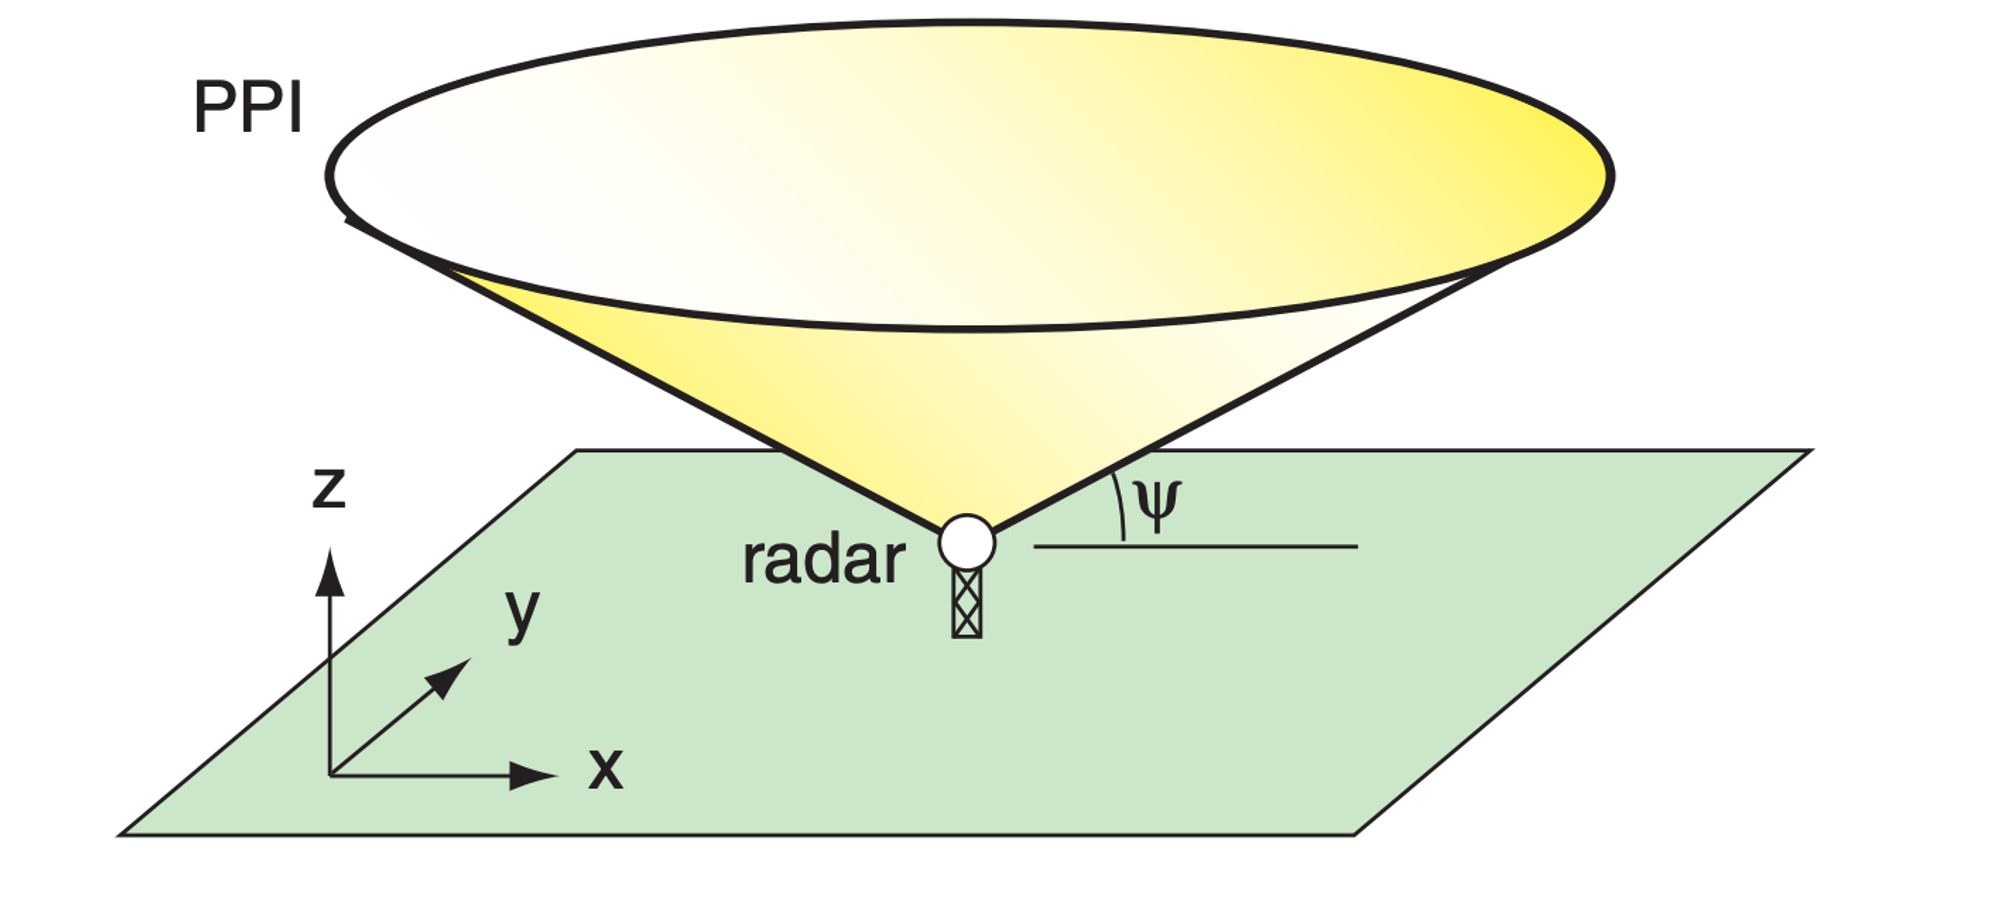
\includegraphics[width=0.85\textwidth]{Images/2.1-ppi.png}
    \caption{Sản phẩm quét tròn với góc nâng cố định (Plan-Position Indicator - PPI) - \cite{2022Weather}}
    \label{fig:ppi}
\end{subfigure}

\begin{subfigure}{\textwidth}
    \centering
    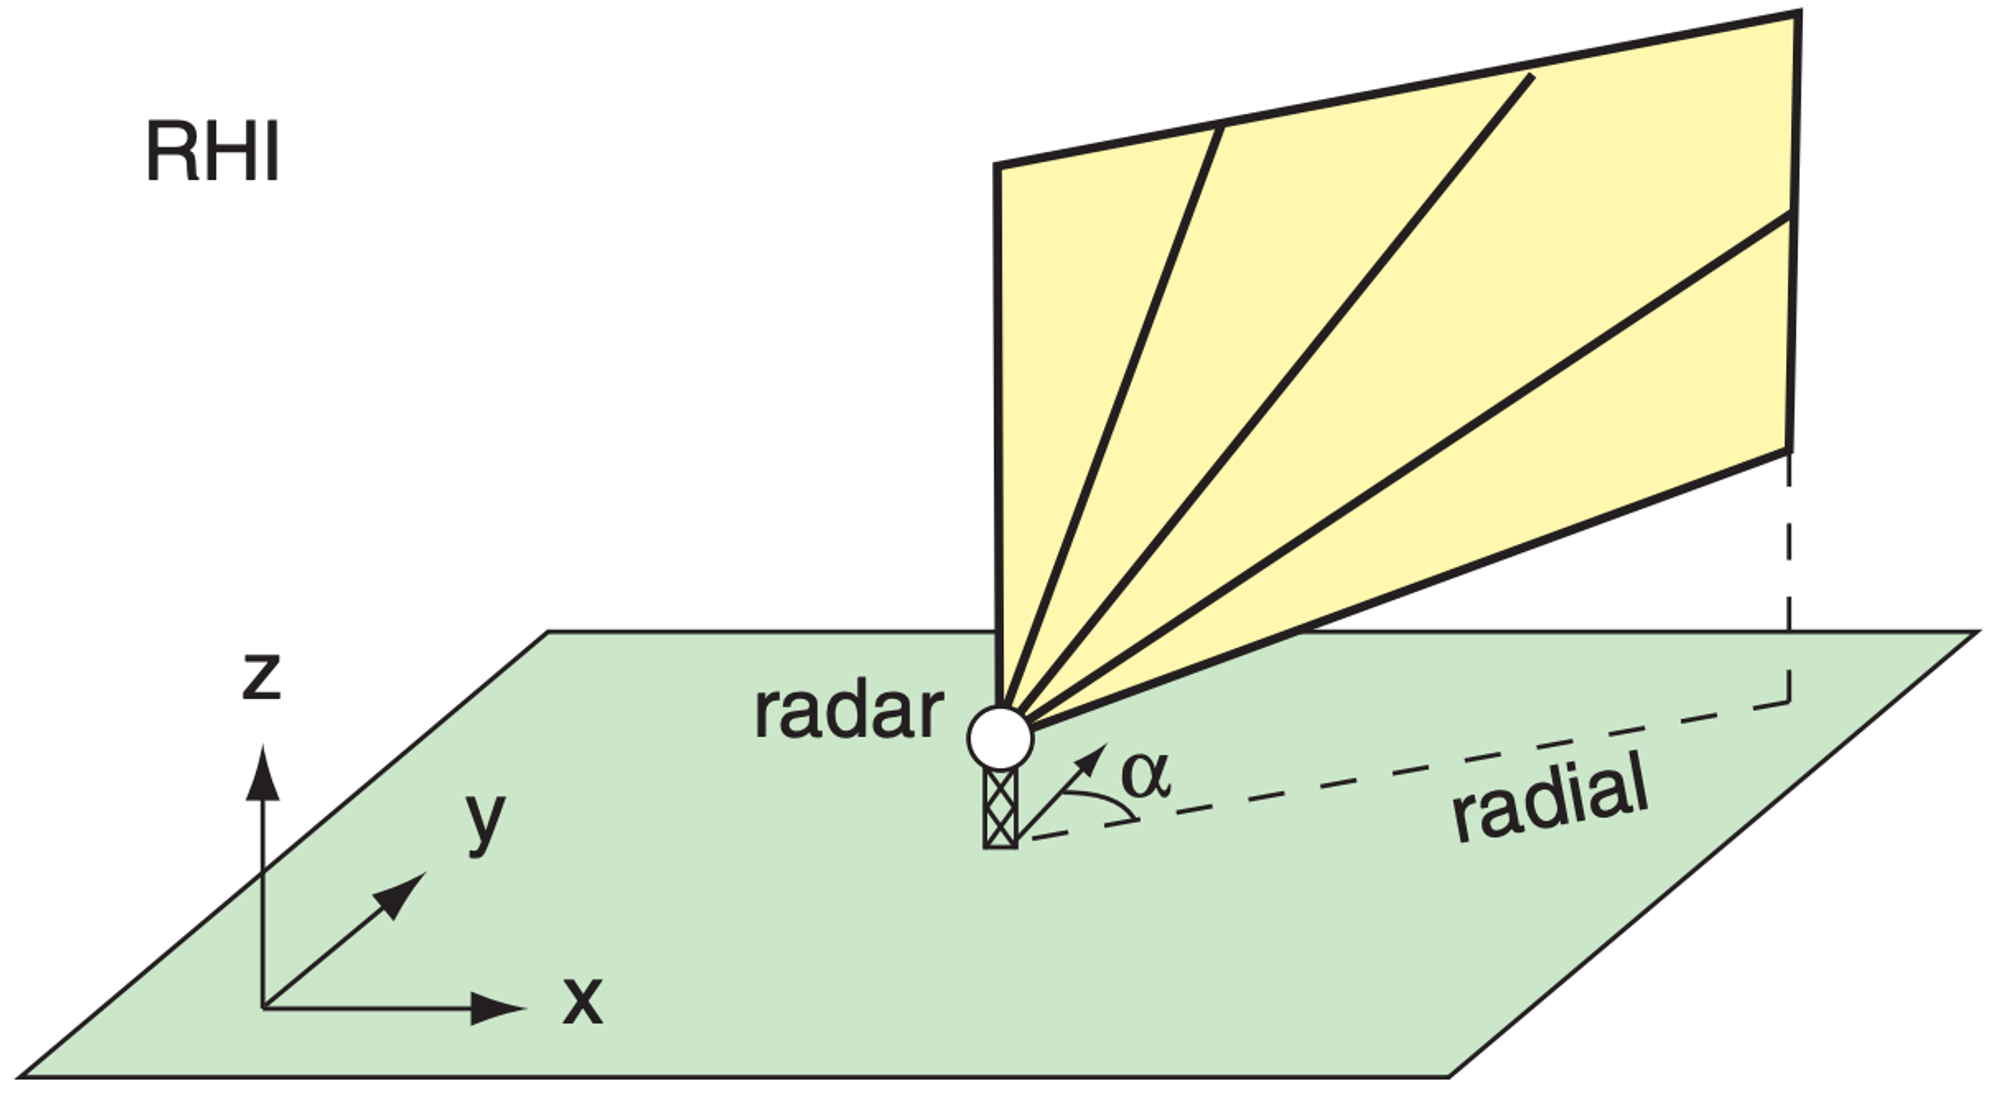
\includegraphics[width=0.85\textwidth]{Images/2.1-rhi.png}
    \caption{Sản phẩm quét thẳng đứng ở một gốc phương vị nhất định (Range Height Indicator) - \cite{2022Weather}}
    \label{fig:rhi}
\end{subfigure}

\end{figure}

Đối với biểu diễn PPI, radar sẽ quét toàn bộ góc hướng, nhưng chỉ ở một góc nâng nhất định. Kết quả thu được tương tư một bản đồ trên mặt phẳng. Với RHI, radar sẽ giữ nguyên góc hướng nhưng thay đổi về góc nâng. Kết quả thu được giúp người xem có cái nhìn rõ nét hơn về chiều cao, kích thước của hiện tượng khí tượng.

\begin{figure}[H]
    \centering
    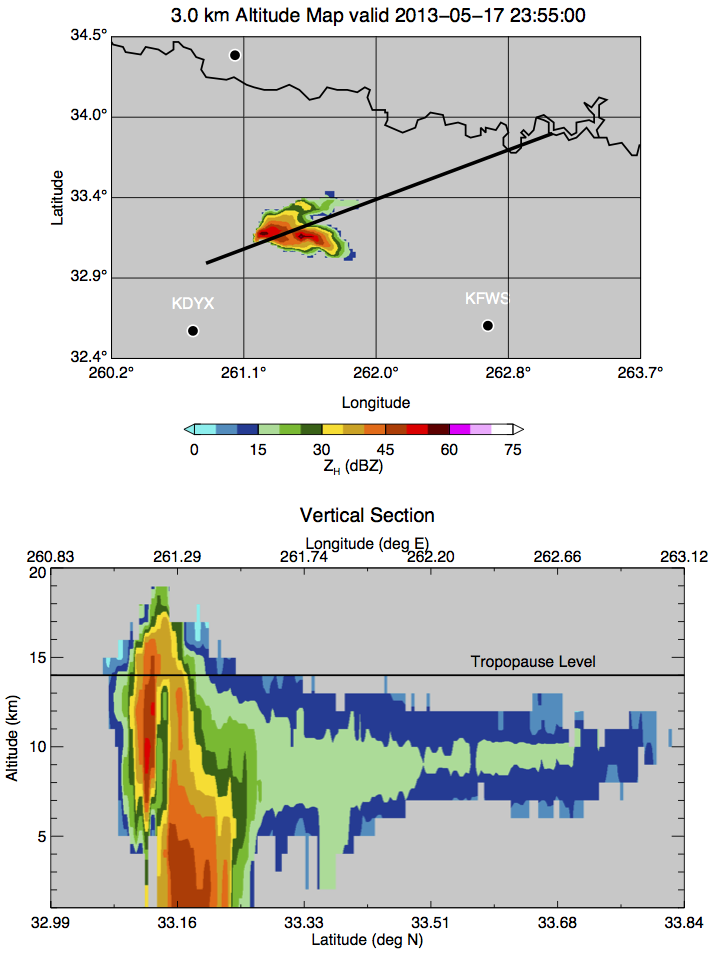
\includegraphics[width=\linewidth]{Images/2.1-ppi-and-rhi.png}
    \caption{So sánh kết quả thu được từ phương pháp PPI và RHI - \cite{stackexchange-ppi-rhi}}
    \label{fig:ppi-and-rhi}
\end{figure}

\subsubsection{Phương trình Radar và độ phải hồi vô tuyến}
Tại một thời điểm, radar sẽ phát ra một luồng sóng trong khoảng thời gian ngắn ($\Delta t = 0.5 - 10 \mu s$). Lúc này, tuỳ thuộc mật độ các phân tử tự do trong không khí (hơi nước, khói bụi, ...), năng lượng của bước sóng này sẽ bị hấp thụ một phần. Cường độ bước sóng mà radar nhận được sẽ nhỏ hơn cường độ sóng ban đầu. Tỉ lệ này được thể hiện thông qua \textbf{Phương trình radar} \cite{2022Weather}:

\[
    \left[ \frac{P_R}{P_T} \right]=\left[ b \right]\cdot\left[ \frac{|K|}{L_a} \right]^2\cdot\left[ \frac{R_1}{R} \right]^2\cdot\left[ \frac{Z}{Z_1} \right]
\]
\vspace{0.5cm}

Trong đó, các biến của phương trình gồm có:
\begin{itemize}
    \item $|K|$ không có đơn vị:
    \begin{itemize}
        \item $|K|^2 \approx 0.93$ cho các hạt nước lỏng
        \item $|K|^2 \approx 0.208$ cho tinh thể băng
    \end{itemize}
    \item $R (\text{km})$: khoảng cách
    \item $R_1 = \sqrt{Z_1 \cdot c \cdot \Delta t / \lambda^2}$: hệ số khoảng cách
    \item $Z$: Hệ số phản hồi vô tuyến của Radar
    \item $Z_1 = 1 \text{ mm}^6 \text{ m}^{-3}$: hệ số đơn vị phản hồi vô tuyến
\end{itemize}

Từ phương trình Radar, ta suy ra được công thức tính độ phản hồi vô tuyến:
\vspace{0.5cm}
\[
    \text{dBZ} = 10\left[ \log\left( \frac{P_R}{P_T} \right) + 2 \log\left( \frac{R}{R_1} \right) - 2\log\left| \frac{K}{L_a} \right| - \log\left( b \right) \right]
\]
\vspace{0.5cm}

Các nhà khí tượng thuỷ văn học thường quan tâm đến con số này vì nó tỉ lệ thuận với mức độ giáng thuỷ (precipitation).
\vspace{0.5cm}

\begin{table}[h]
    \centering
    \begin{tabular}{|c|c|}
        \hline
        Giá trị (dBZ) & Thời tiết \\
        \hline
        -28 & Sương mù \\
        -12 & Không khí trong lành \\
        25 - 30 & Tuyết khô / mưa nhẹ \\
        40 - 50 & Mưa lớn \\
        75 & Mưa đá khổng lồ \\
        \hline
    \end{tabular}
    \vspace{1em}
    \caption{Tương quan hệ số phản xạ của radar và giáng thuỷ - \citet{2022Weather}}
\end{table}

\begin{figure}[H]
    \centering
    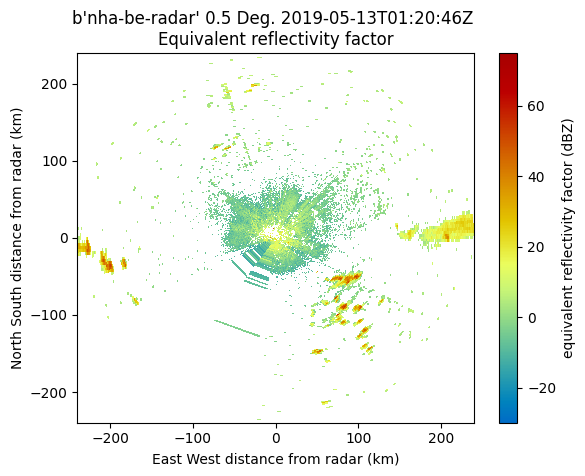
\includegraphics[width=0.75\textwidth]{Images/2.1-reflectivity_nhabe.png}
    \vspace{1em}
    \caption{Minh hoa hệ số phản xạ từ dữ liệu radar Nhà Bè}
    \label{fig:reflectivity-nhabe}
\end{figure}


\subsubsection{Vận tốc xuyên tâm}

\begin{figure}[H]
    \centering
    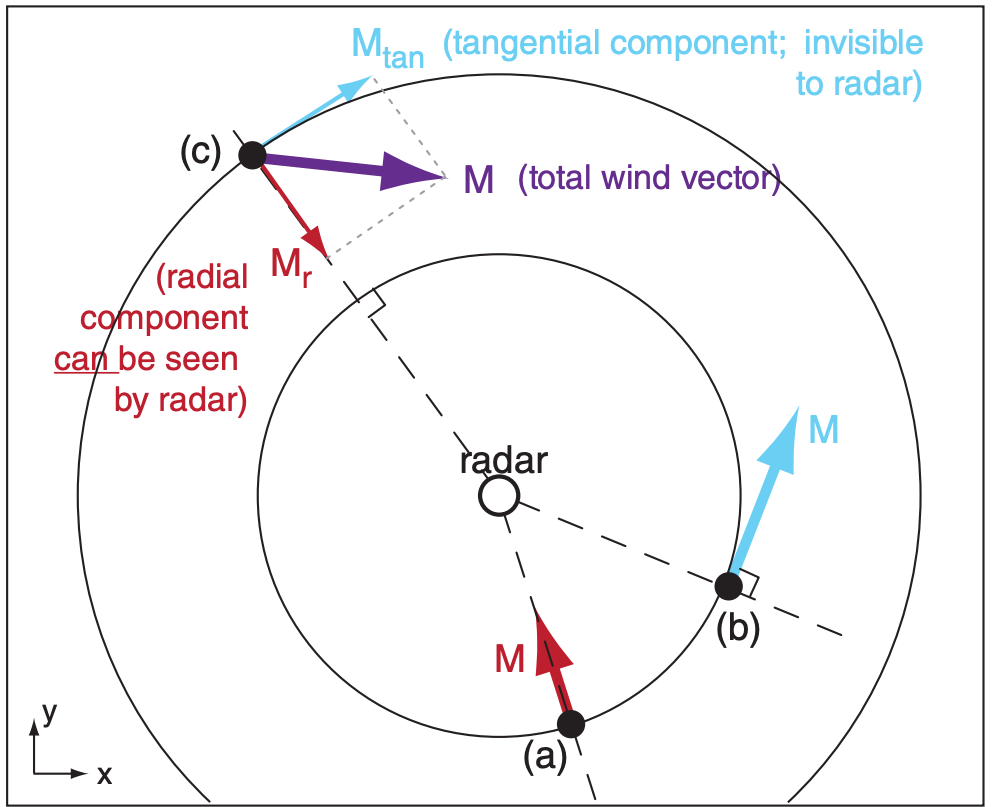
\includegraphics[width=.55\textwidth]{Images/2.1-radial-velocity.png}
    \vspace{2em}
    \caption{Minh hoạ các tình huống vận tốc mà radar Doppler có thể quan sát. (a) Phương của gió trùng tại M trùng với đường kính đường tròn có tâm tại radar, radar có thể xác định được vận tốc tại đây. (b) Phương của gió trùng với tiếp tuyến của đường tròn, radar không thể xác định được vận tốc. \(c\) Phân tích hướng gió tại M thành 2 vận tốc vuông góc nhau, radar chỉ xác định được vector vận tốc theo $M_r$}
    \label{fig:radial-velocity}
\end{figure}

Khi các sóng vô tuyến từ các radar Doppler này truyền đến các phân tử trong không khí, sự chuyển dịch vị trí của các hạt này làm lệch pha giữa tín hiệu truyền đi và tín hiệu nhận lại được. Các radar sẽ căn cứ vào thông tin này để tính toán vận tốc gió tại các điểm trong không gian.